\newpage
\section{Resultados}
\subsubsection{Regresi\'on Lineal}
Sin la introducci\'on de par\'ametros se alcanzo el 0.082 de sme:

\begin{figure}[h!]
	\centering
	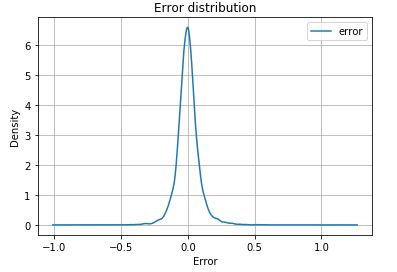
\includegraphics[width=0.8\linewidth]{Figure/LinearRegresionED_Results.JPG}
	\caption{Regresi\'on Lineal: distribuci\'on de error} 
	\label{fig:LinearRegresionED_Results}
\end{figure}

\begin{figure}[h!]
	\centering
	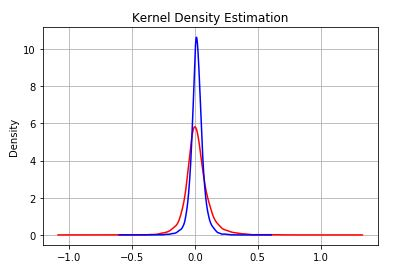
\includegraphics[width=0.8\linewidth]{Figure/LinearRegresionKernel_Results.JPG}
	\caption{Regresi\'on Lineal: Estimaci\'on de densidad del n\'ucleo} 
	\label{fig:LinearRegresionKernel_Results}
\end{figure}

\begin{figure}[h!]
	\centering
	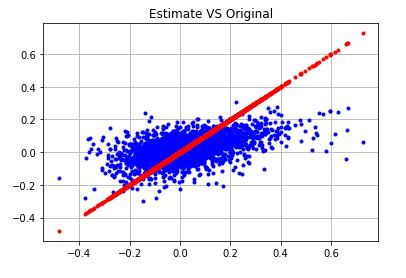
\includegraphics[width=0.8\linewidth]{Figure/RegresionLineal_Results.JPG}
	\caption{Regresi\'on Lineal: Estimate vs Original} 
	\label{fig:LinearRegresionKernel_Results}
\end{figure}
\\

\newpage
\subsubsection{Decision Tree}
El mejor m\'odelo se obtuvo con los siguientes par\'ametros con un sme de 0.093583:
\begin{lstlisting}[language=Python]
{	'criterion': mae		
	'splitter': best	
	'max_depth':2.0		
	'max_features':0.24
}\end{lstlisting}
\\
Las siguientes gr\'aficas corresponden a los resultados con los respectivos par\'ametros y usando los set de pruebas:
\begin{figure}[h!]
	\centering
	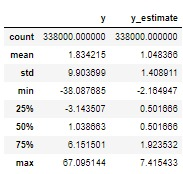
\includegraphics[width=0.3\linewidth]{Figure/dtr_decription.jpeg}
	\caption{Data description (DT)} 
	\label{fig:dt_ed}
\end{figure}
\\
\begin{figure}[h!]
	\centering
	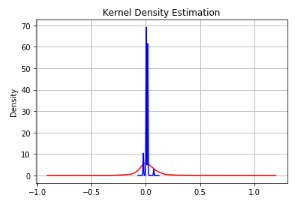
\includegraphics[width=0.8\linewidth]{Figure/dtr_kerneldensity.jpeg}
	\caption{Kernel density (DT)} 
	\label{fig:dt_kd}
\end{figure}
\\
\begin{figure}[h!]
	\centering
	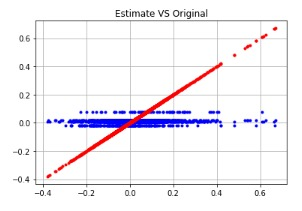
\includegraphics[width=0.8\linewidth]{Figure/dtr_estimorg.jpeg}
	\caption{Estimate vs Original(DT)} 
	\label{fig:dt_eo}
\end{figure}

\newpage
\subsubsection{XGBoost}
El mejor m\ódelo se obtuvo con los siguientes par\'ametros con un sme de 0.062:
\begin{lstlisting}[language=Python]
xgb_grid.best_params_
{'colsample_bytree': 0.7, 
'learning_rate': 0.07, 
'max_depth': 5, 
'min_child_weight': 4, 
'n_estimators': 100, 
'nthread': 4, 
'objective': 'reg:linear', 
'silent': 1, 
'subsample': 0.7}
\end{lstlisting}
Las siguientes gr\'aficas corresponden a los resultados con los respectivos par\'ametros y usando los set de pruebas:
\begin{figure}[h!]
	\centering
	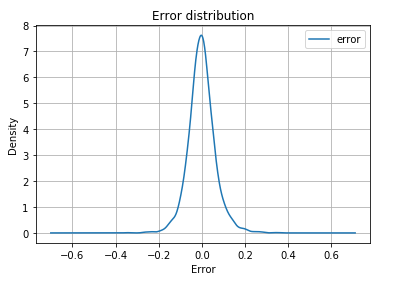
\includegraphics[width=0.8\linewidth]{Figure/xgbregresor_results.png}
	\caption{Error distribution(XGB)} 
	\label{fig:xgbregresor}
\end{figure}
\begin{figure}[h!]
	\centering
	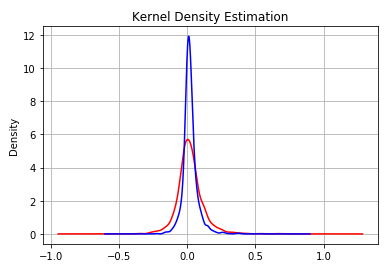
\includegraphics[width=1\linewidth]{Figure/xgbregresorKernel_results.png}
	\caption{Error distribution(XGB)} 
	\label{fig:xgbregresorKernel_results}
\end{figure}
\begin{figure}[h!]
	\centering
	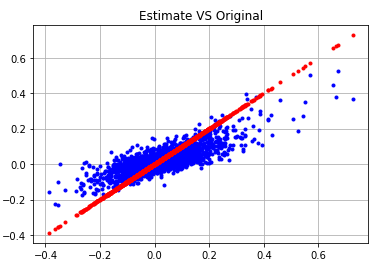
\includegraphics[width=0.8\linewidth]{Figure/xgbregresorEstimation_results.png}
	\caption{Error distribution(XGB)} 
	\label{fig:xgbregresorEstimation_results}
\end{figure}
\\
\\
\newpage
\subsubsection{Naive Bayes}
Best parameter:
smoothing: 307

Las siguientes gr\'aficas corresponden a los resultados con los respectivos par\'ametros y usando los set de pruebas:
\begin{figure}[h!]
	\centering
	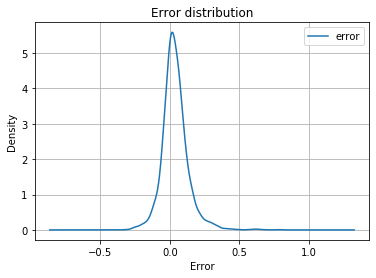
\includegraphics[width=0.8\linewidth]{Figure/nb_error_distribution.png}
	\caption{Error Distribution (Naive Bayes)} 
	\label{fig:nb1}
\end{figure}

\begin{figure}[h!]
	\centering
	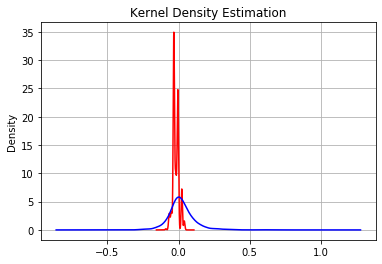
\includegraphics[width=0.8\linewidth]{Figure/nb_density_estimation.png}
	\caption{Density Estimation (Naive Bayes)} 
	\label{fig:nb1}
\end{figure}

\begin{figure}[h!]
	\centering
	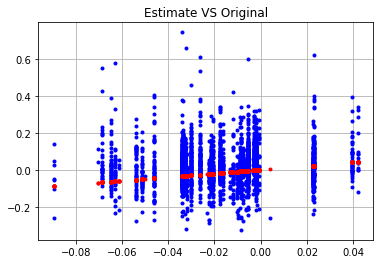
\includegraphics[width=0.8\linewidth]{Figure/nb_estimate_vs_original.png}
	\caption{Estimation vs Original (Naive Bayes)} 
	\label{fig:nb1}
\end{figure}\\

\newpage
\subsubsection{Support Vector Machines Regressor}
\p{El mejor m\'odelo se obtuvo con los siguientes par\'ametros con un sme de 0.093:
\begin{lstlisting}[language=Python]
{'kernel':'poly', 
 'degree':'2', 
 'gamma':'0.55', 
 'coef0':'0.1', 
 'C':'34', 
 'epsilon':'0.2'
}
\end{lstlisting}{}
Las siguientes gr\'aficas corresponden a los resultados con los respectivos par\'ametros y usando los set de pruebas:
\begin{figure}[h!]
	\centering
	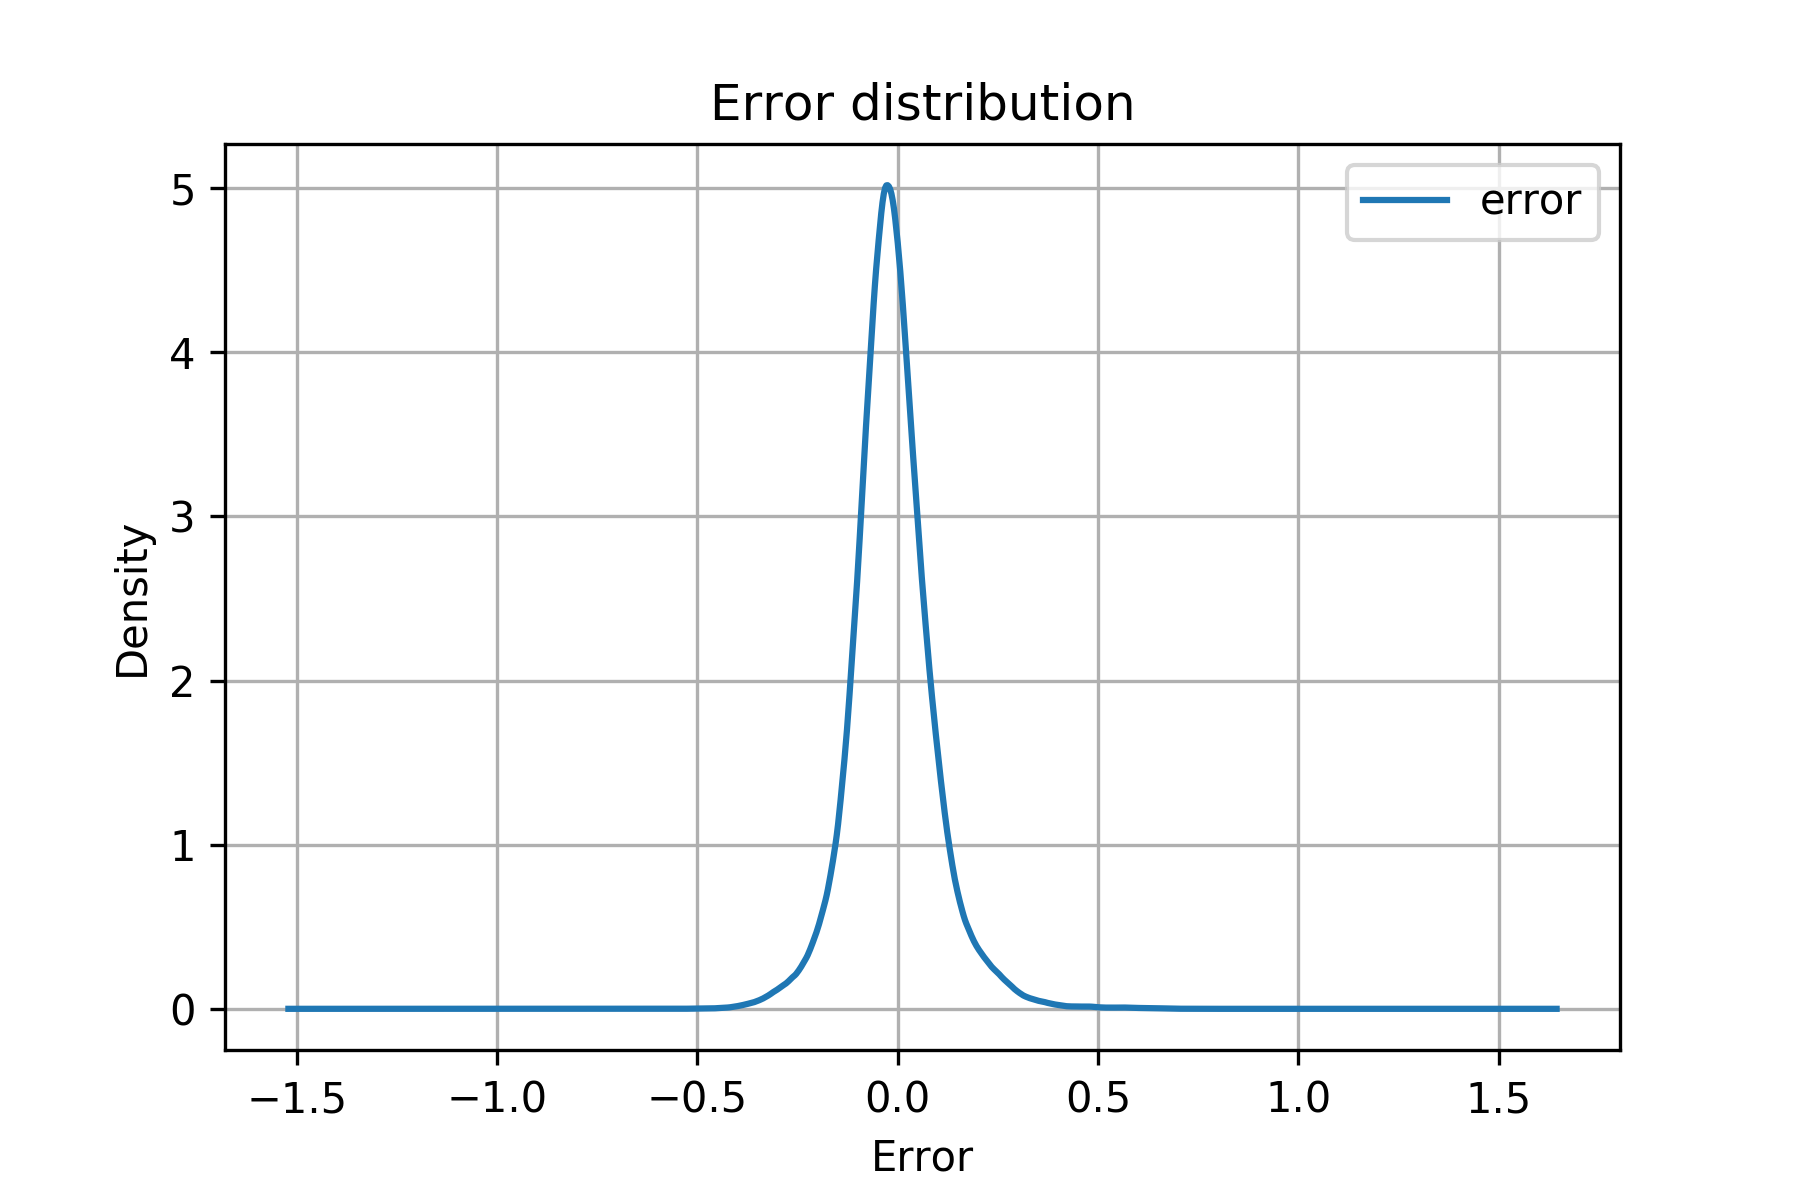
\includegraphics[width=0.8\linewidth]{Figure/svmr_errordist.png}
	\caption{Error Distribution (SVMR)} 
	\label{fig:svmr_ed}
\end{figure}

\begin{figure}[h!]
	\centering
	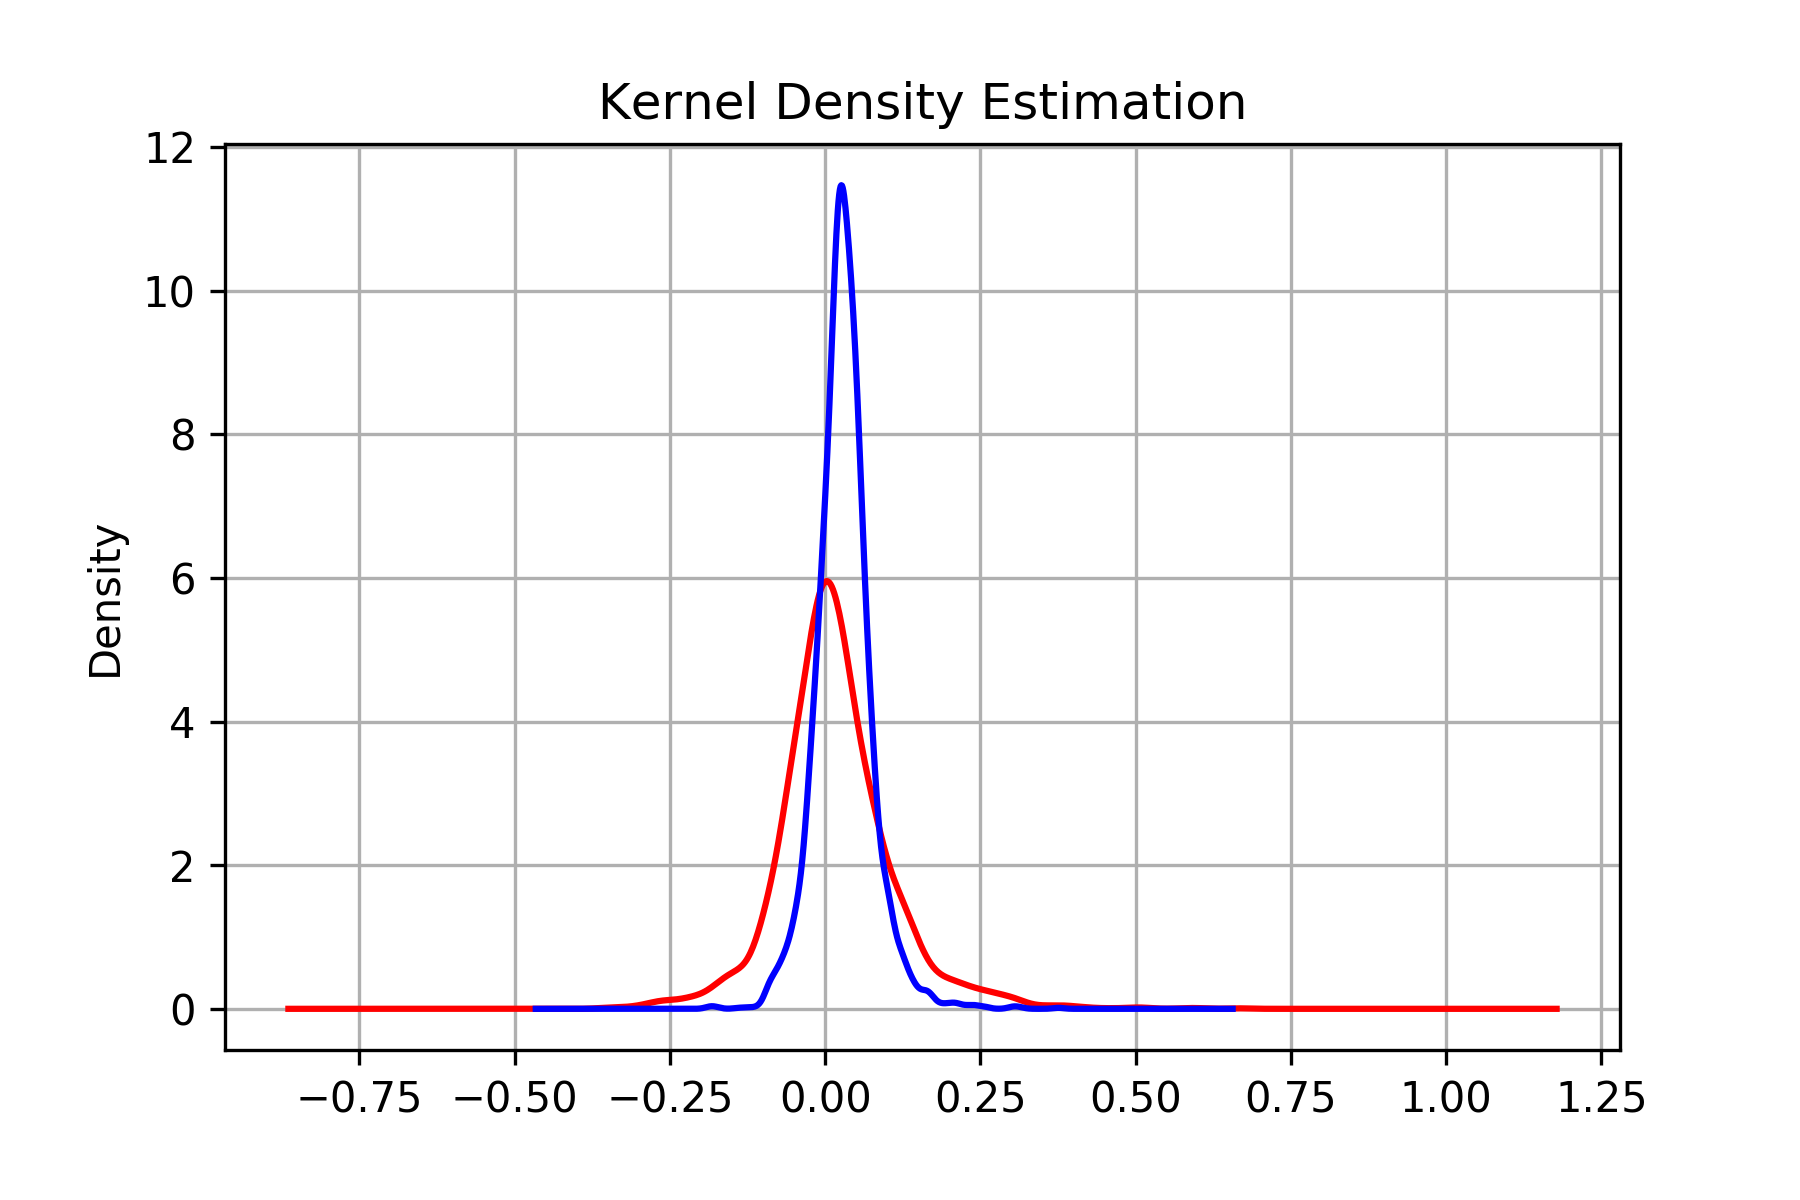
\includegraphics[width=0.8\linewidth]{Figure/svmr_kerneldensity.png}
	\caption{Kernel density (SVMR)} 
	\label{fig:svmr_kd}
\end{figure}

\begin{figure}[h!]
	\centering
	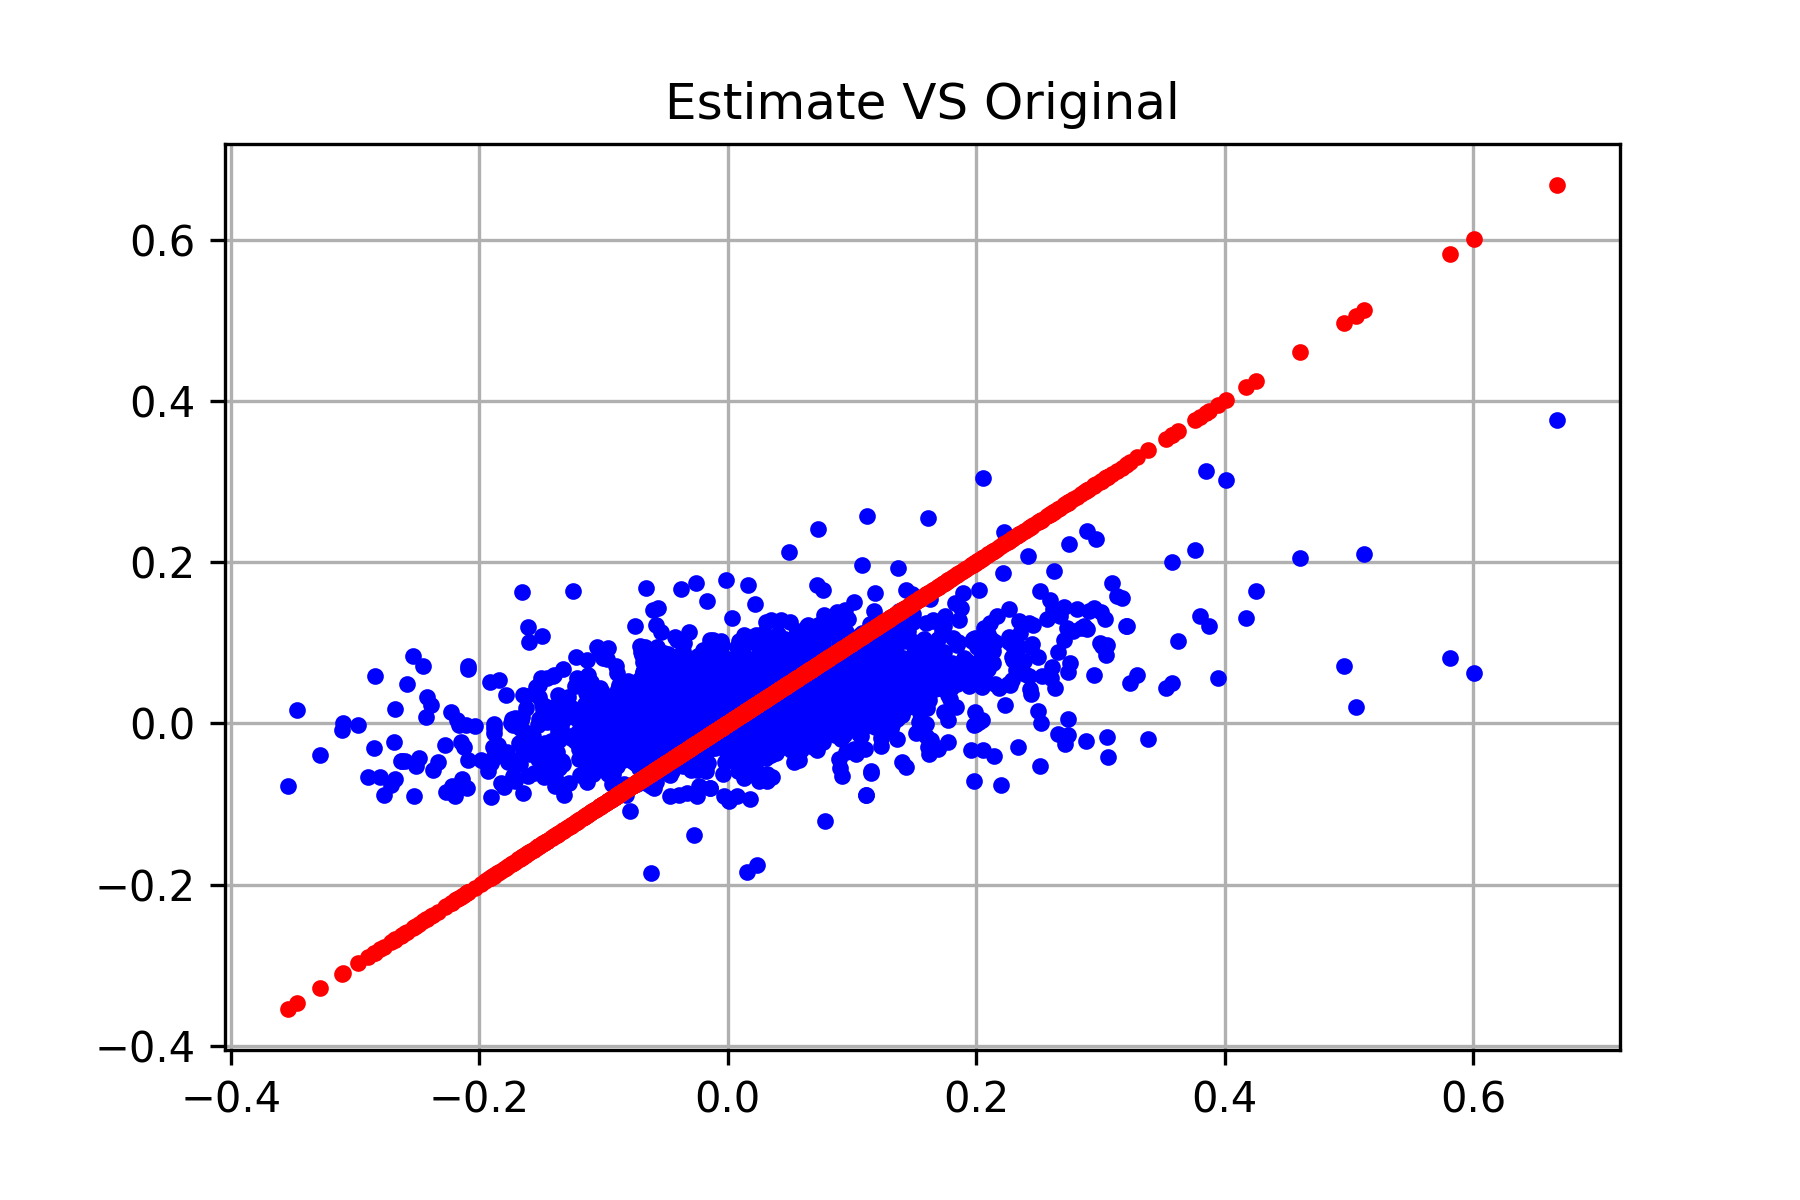
\includegraphics[width=1\linewidth]{Figure/svmr_estiorg.png}
	\caption{Estimate vs Original(SVMR)} 
	\label{fig:svmr_eo}
\end{figure}
} \\

\newpage